% !TEX root =  main.tex
\newpage
\chapter{Application design} \label{ch:sw_design}
The VPP application is implemented in object-oriented Python. The static structure and runtime behavior is det

\section{Static structure}

\begin{figure}[H]
    \centering
    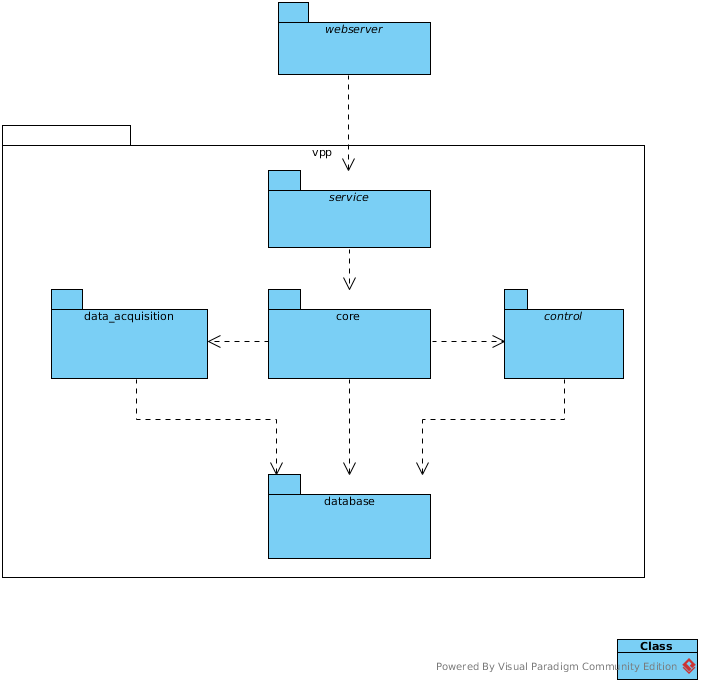
\includegraphics[width=0.5\textwidth]{figures/class_overview}
    \caption{Overview of packages}
    \label{figureClassDiagram}
\end{figure}

The application is roughly structured in a layered architecture with the \texttt{database} as the bottom layer and the \texttt{core} and \texttt{data\_acquisition} packages as the domain layer. A \texttt{service} package could be added as the top layer, providing an external interface. The packages are explained in detail below.


\subsubsection{Package \texttt{vpp.core}}

\begin{figure}[H]
    \centering
    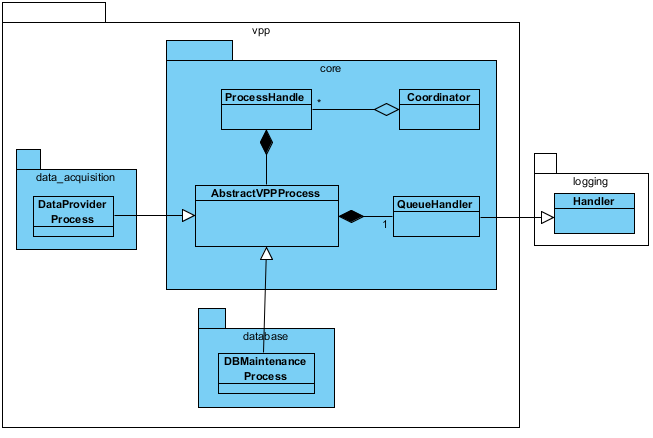
\includegraphics[width=\textwidth]{figures/class_core}
    \caption{Package \texttt{core}}
\end{figure}

\texttt{Coordinator} is called by \texttt{start\_server.sh} and launches the entire application. Mainly, it instantiates the \texttt{DataProviderProcess} and the \texttt{DBMaintenanceProcess}. The processes are each wrapped in a \texttt{ProcessHandle} which handles process launch and termination and receives log messages from the underlying  \texttt{AbstractVPPProcess}. That is, all log messages are communicated (using Python interprocess message queues) to the main process which outputs to \texttt{logs/console.log}.


\subsubsection{Package \texttt{vpp.data\_acquisition}}

\begin{figure}[H]
    \centering
    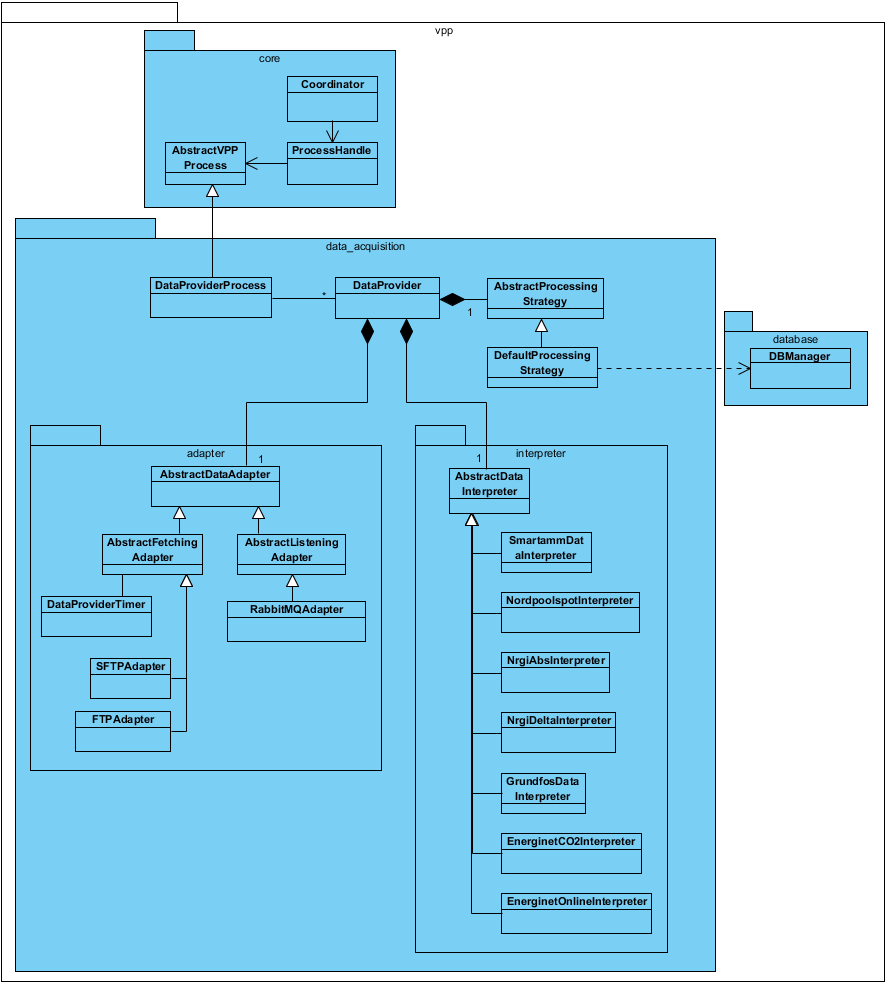
\includegraphics[width=\textwidth]{figures/class_data_acquisition}
    \caption{Package \texttt{data\_acquisition}}
\end{figure}

This package contains the framework for connecting to sources of measurement and prediction data. The \texttt{DataProviderProcess} launches a \texttt{DataProvider} for each configured \texttt{.ini}-file as described in \ref{sec:data_provider_config}. Each \texttt{DataProvider} instance employs a suitable \texttt{DataAdapter}. The \texttt{FetchingAdapter}s employ a \texttt{DataProviderTimer} that will wake up according to configuration and execute data retrieval and processing. The \texttt{ListeningAdapter} will launch a thread that continuously listens for messages and processes them as they are received. Thus, each data provider does all processing in its own thread.

The \texttt{DataAdapters} handle communication with the data source and extract a raw string that is then passed to the configured \texttt{DataInterpreter}. The interpreter parses the string and outputs data as Python dictionaries to the \texttt{ProcessingStrategy} which interacts with a \texttt{DBManager} to store the data.


\subsubsection{Package \texttt{vpp.database}}

This package contains the code that interfaces directly with the database. 

\begin{figure}[H]
	\centering
	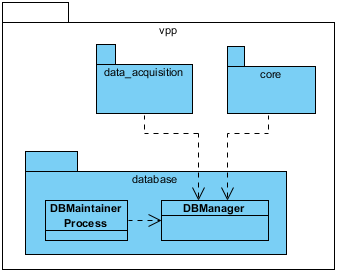
\includegraphics[width=0.5\textwidth]{figures/class_db}
	\caption{Package \texttt{database}}
	\label{}
\end{figure}

\texttt{DBMaintainerProcess} wakes up in accordance with the period specified in \texttt{config.ini} and instantiates  \texttt{DBMaintenance} that runs maintenance on the database, implementing the Rolling Window strategy.

\texttt{DBManager} provides an interface to the database. It relies on \texttt{SchemaManager} which implements initialization of the database schema as well as creation and lookup of subtables for the Rolling Window scheme. The \texttt{measurement} and \texttt{prediction} tables and their subtables are implemented directly in SQL, but the rest of the schema is implemented using the object-relational mapper (ORM) framework SQLAlchemy.

\newpage
\section{Runtime behavior}

Separate Python processes are deployed to enable concurrent processing. Using processes instead of threads is necessary to fully utilize multiple cores, since Python employs a \emph{Global Interpreter Lock} which prevents threads within the same Python interpreter from executing concurrently. Using processes mitigates this as each process will run with its own interpreter. For this prototype, the multiprocessing could probably have been omitted in favor of simpler multithreading since CPU load has not been an issue at all.

The runtime creation of processes within the main server application is shown below:
\begin{figure}[H]
    \centering
    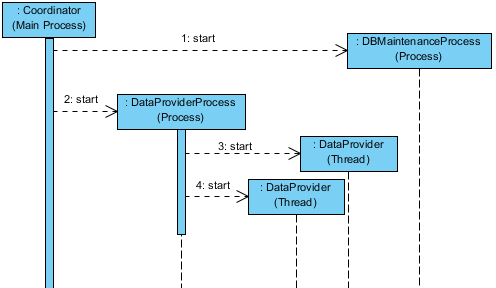
\includegraphics[width=\textwidth]{figures/seq_diagram_init}
    \caption{Simplified sequence diagram of process and thread creation}
\end{figure}

In the diagram above, the \texttt{ProcessHandle} class is omitted for clarity.


\newpage
\subsection{Data acquisition}
\begin{figure}[H]
    \centering
    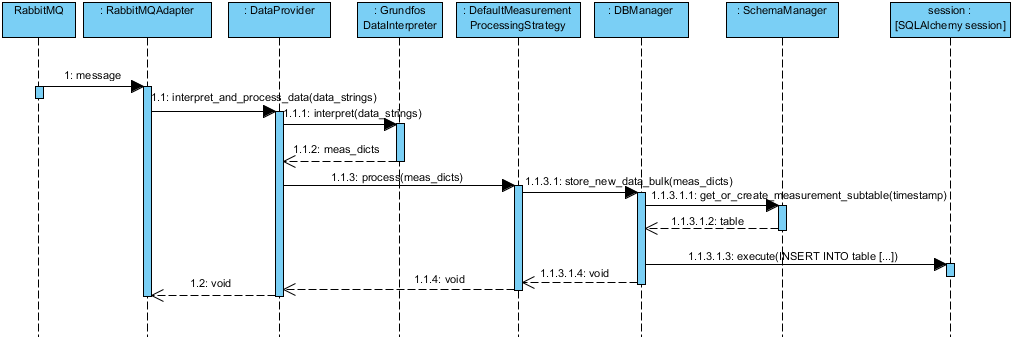
\includegraphics[width=0.9\textheight, angle=90]{figures/data_acq_seq_diagram}
    \caption{Sequence diagram of receiving measurements from a RabbitMQ}
\end{figure}


